%\section{Numerical Experiments}

We verify our theoretical claims 
on synthetic generative priors. We  consider  2-layer generative networks with Relu activation functions, hidden layer of dimension $n_1 = 250$, output dimension $n = 1700$ and varying number of latent dimension $k \in [10, 30, 70]$. 
We randomly sample the weights of the matrix independently from $\mathcal{N}(0, 2/n_i)$, which removes that $2^d$ dependence in Theorem \ref{thm:main_rand}.
We then consider data $Y$ according the spiked models \eqref{eq:wishart_Y} and \eqref{eq:wigner_Y}, where $\xstar \in \R^k$ is chosen so that $\ystar = G(\xstar)$ has unit norm. For the Wishart model we vary the samples $N$ while for the Wigner model we vary the noise level $\nu$ so that the following quantities remain constant for the different networks (latent dimension $k$):
\[
\theta_{\text{\tiny WS}}:=\sqrt{k\log(n_1^2\,n)/N}, \qquad  \theta_{\text{\tiny WG}}:=\nu \sqrt{k\log(n_1^2\,n)/n}
\]
We then plot the reconstruction error 
given by $\|G(x) - \ystar \|_2$ against $\theta_{\text{\tiny WS}} \approx  \sqrt{\frac{k}{N}}$ and $\theta_{\text{\tiny WG}} \approx \nu\sqrt{\frac{k}{n}}$.
As predicted by Theorem \ref{thm:main_rand} the errors scale linearly with respect to these control parameters, and moreover all the plots overlap confirming that these rates are tight with respect to the order of $k$. 



\begin{figure}[h]%
	\centering
	\subfloat{{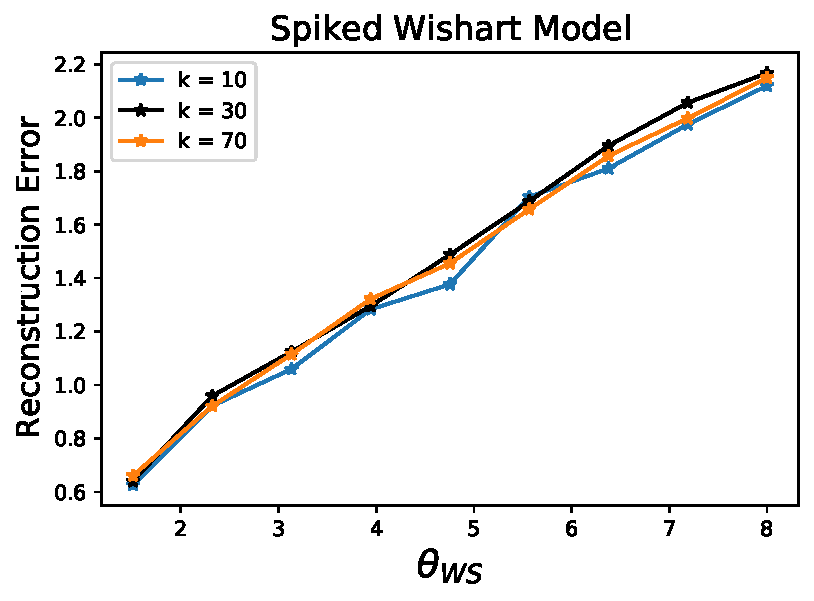
\includegraphics[width=6.5cm]{imgs/MSE_WS_new.pdf} }}%
	\qquad
	\subfloat{{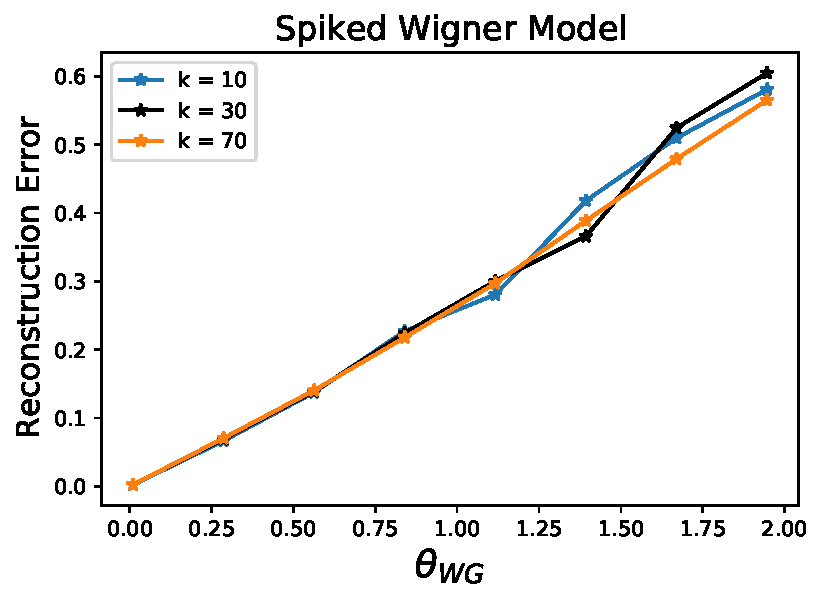
\includegraphics[width=6.5cm]{imgs/MSE_WG_new2.pdf} }}%
	\caption{Reconstruction error for the recovery of a spike $\ystar = G(\xstar)$ in Wishart and Wigner model with random generative network priors. Average over 50 random drawing of the network weights and samples. These plots demonstrate that the reconstruction error follow closely our theory.}%
	\label{fig:example}%
\end{figure}

%\begin{figure}[h]
%	\centering
%	\includegraphics[width=0.9\linewidth]{imgs/WIG_3Lvs2L_150dpi}
%	\caption{MSE as a function of the scaling parameter}
%	\label{fig:WIG_3Lvs2L_150dpi}
%\end{figure}